\documentclass{article}
\usepackage[a4paper, margin=1in]{geometry}
\usepackage[utf8]{inputenc}
\usepackage{graphicx}
\usepackage{url}
\usepackage{array}
\usepackage{hyperref}
\usepackage[table,dvipsnames]{xcolor}
\usepackage{afterpage}
\usepackage{fix-cm}
\usepackage{lipsum}
\usepackage{sectsty}
\usepackage{tabularx}
\usepackage{tabto}
\usepackage[export]{adjustbox}


\definecolor{FSBlue}{HTML}{13284c}
\definecolor{FSRed}{RGB}{177, 16, 44}

\usepackage{newtxmath}

\sectionfont{\color{FSRed}}
\subsectionfont{\color{FSBlue}}


\begin{document}

\newgeometry{top=20mm, left=10mm, bottom=20mm} 
\pagecolor{white}\afterpage{\nopagecolor}



\includegraphics[width=10cm]{images/TH_Koeln_Logo.svg.png}
% \begin{center}
\vspace{2in}

\fontsize{50}{50}\selectfont \textcolor{FSBlue}{\textbf{MA2 Team 24}}

\fontsize{30}{30}\selectfont \textcolor{FSBlue}{\textbf{Dokumentation}}

\vspace{10mm}
\LARGE\textcolor{FSBlue}{\textbf{Thema: Simplex}}

\vspace{0.5in}

\Large\textcolor{FSBlue}{Lukas Fey, Mike Springer, Tobias Mai, Lennart van Gisteren, Vanessa Pater}

\vspace{3in}



\thispagestyle{empty}
% \end{center}
\restoregeometry   
\newpage

\input{sections/Einführung}

\section{Methoden}

Die drei Simplex-Methoden sind der primale Simplex, der duale Simplex und die Big M Methode. Zum optimieren unseres Problems haben wir den primalen Simplex verwendet.\\\\
Der duale Simplex-Algorithmus wird angewendet, wenn die Werte der rechten Seite der Nebenbedingungen negativ sind. Der primale Simplex-Algorithmus wird angewendet, wenn alle Werte der rechten Seite positiv sind. Der duale Simplex-Algorithmus führt zu einer zulässigen Ausgangslösung, der primale Simplex-Algorithmus zu einer optimalen Lösung. Nach Anwendung des dualen Simplex-Algorithmus kann der primale Simplex-Algorithmus angewendet werden, um eine optimale Lösung zu erhalten. 
\\




\section{Geschichtlicher Hintergrund und Begriffe}
\subsection{Die Geschichte}
Der russische Mathematiker L. V. Kantorovich veröffentlichte 1939 das Buch "Mathematische Methode in der Organisation und Planung der Produktion", welche mithilfe von mathematischen Modellen die Kosteneffizienz in der Produktion eines Betriebes steigern soll. Die Arbeit Kantorovichs ist insofern bedeutend, da er als erstes erkannte, dass bestimmte Arten der Produktion, definierte mathematische Strukturen besitzen, die numerisch gelöst werden können. Allerdings wurde zu jener Zeit die Bedeutung dieser Arbeit nicht in vollem Umfang erkannt. Mitte der 1940-er Jahre wurde Georg Dantzig bewusst, dass sich viele praktische ökonomische Beschränkungen bei der Modellierung von Planungsaufgaben durch lineare Ungleichungen beschreiben lassen. Er ersetzte erstmals bewusst die bis dahin geltenden Regeln zur Lösung von Planungsproblemen durch eine Zielfunktion und Nebenbedingungen, in Form von Gleichungen und Ungleichungen. Dadurch entstand eine klare Trennung zwischen dem Ziel der Optimierung, der zulässigen Lösungsmenge und den Mitteln zur Lösung des Problems. 1950 wurde der Simplex-Algorithmus zum ersten Mal mit Computern zur Lösung des Transportproblems genutzt. Die Nutzung von Computern in Betrieben wuchs immens. Lineare Optimierung wurde für die Industrie zwischen den 1955-1960 wichtiger und sie wurde beispielsweise vom Management als Verfahren zur Optimierung der Effizienz des Betriebes genutzt. Die Öl-Industrie und die Landwirtschaft waren Wirtschaftszweige, welche die Lineare Optimierung besonders effizient anwenden konnten. Seit 1957 wuchsen die Anwendungsbereiche immer weiter. 
\\
\subsection{Wichtige Begriffe/Das Verfahren}

Damit der Simplex-Algorithmus angewendet werden kann, müssen Nebenbedingungen und eine Zielfunktion bestimmt werden. Daraufhin muss entschieden werden, ob die Zielfunktion maximiert oder minimiert wird. Danach wird das Problem in eine Art Matrixform – das Simplex-Tableau – übertragen. Mithilfe von sogenannten Schlupfvariablen s1 und s2 wird es möglich, dass aus den beiden Ungleichungen zwei Gleichungen gebildet werden. Es wird jeweils nur eine Schlupfvariable pro Zeile genutzt, sodass sie in der Simplex Tabelle eine Einheitsmatrix bilden. Die Zielfunktion des Algorithmus wird vorzugsweise an der untersten Stelle der Tabelle eingetragen. Neben den Schlupfvariablen gibt es noch Basisvariablen. Als Basisvariable werden die x- Werte in den Nebenbedingungen bezeichnet. Die Werte, die in der Zielfunktion anstelle der Schlupfvariablen stehen, werden als Schattenpreis bezeichnet. Das bedeutet, wenn die Menge für x1 um 1 erhöht wird, wirkt sich das auf den Gesamtwert um den Wert bei dem Schattenpreis aus. Die Pivotspalte sowie die Pivotzeile sind jede Zeile und Spalten, die beim Algorithmus ausgewählt werden, um das Pivotelement zu bestimmen. Im weiteren Verlauf wird anhand eines Beispiels erläutert, wie die Pivotzeile und die Pivotspalte sowie dass Element ausgewählt werden müssen.







\section{Beispiel}
Um das Verfahren zu veranschaulichen, haben wir ein kleines Beispielproblem zusammengebaut, welches wir mithilfe des Simplex Verfahrens lösen.\\~\\
Die Nebenbedingungen für das Problem lauten:\\~\\
\(4x_1+x_2\le3\)\\
\(2x_1+4x_2\le8\)\\~\\
Unter diesen Bedingungen soll die Zielfunktion\\~\\
\(Z = 2x_1+ 3x_2\)\\~\\
maximiert werden\\
\\
\begin{center}
    
\textbf{Schritt 1: \\Ungleichungen zu Gleichungen machen, mithilfe von Schlupfvariablen }\end{center}

\(x_1+x_2+s_1=3\)\\
\(2x_1+6x_2+s_2=8\)\\~\\~\\~\\
\begin{center}
%ab hier sieht man manchmal ein $ vor und hinter einigen Zahlen, dieses startet den "math mode" sodass die Zahl hinter dem x klein und unten ist
\textbf{Schritt 2:\\In Simplex Tableau eintragen}\\\end{center}
\begin{table}[h]
\begin{tabular}{|l|l|l|l|l|l|}
\hline
\rowcolor[HTML]{C0C0C0} 
Zeile                     & $x_1$ & $x_2$ & $s_1$ & $s_2$ & Rechte Spalte \\ \hline
\cellcolor[HTML]{C0C0C0}1 & 1  & 1  & 1  & 0  & 3             \\ \hline
\cellcolor[HTML]{C0C0C0}2 & 2  & 4  & 0  & 1  & 8             \\ \hline
\cellcolor[HTML]{C0C0C0}Z & 2  & 3  & 0  & 0  & 0             \\ \hline
\end{tabular}
\end{table}

\begin{center}\textbf{Schritt 3: \\Pivotelement bestimmen}\end{center}
Hierzu muss der größte Wert der untersten (3.) Zeile rausgesucht werden. Die Spalte, in der sich dieser Wert befindet, ist die Pivotspalte, deren Werte dann mit der Rechten Spalte dividiert werden. Die Zeile, in welcher sich der kleinste Wert ergibt, ist die Pivotzeile. Da, wo Pivotspalte und Pivotzeile einander treffen, befindet sich das Pivotelement.\\
\begin{table}[h]
\begin{tabular}{|
>{\columncolor[HTML]{C0C0C0}}l |
>{\columncolor[HTML]{FFFFFF}}l |
>{\columncolor[HTML]{CBCEFB}}l |
>{\columncolor[HTML]{FFFFFF}}l |
>{\columncolor[HTML]{FFFFFF}}l |
>{\columncolor[HTML]{FFFFFF}}l |l|}
\hline
Zeile & \cellcolor[HTML]{C0C0C0}$x_1$& \cellcolor[HTML]{C0C0C0}$x_2$ & \cellcolor[HTML]{C0C0C0}$s_1$ & \cellcolor[HTML]{C0C0C0}$s_2$ & \cellcolor[HTML]{C0C0C0}Rechte Spalte & \cellcolor[HTML]{C0C0C0}RS/PS \\ \hline
1     & 1                          & 1                          & 1                          & 0                          & 7                                     & 3                             \\ \hline
2     & \cellcolor[HTML]{CBCEFB}2  & \cellcolor[HTML]{FD6864}4  & \cellcolor[HTML]{CBCEFB}0  & \cellcolor[HTML]{CBCEFB}1  & \cellcolor[HTML]{CBCEFB}8             & \cellcolor[HTML]{CBCEFB}2     \\ \hline
Z     & 2                          & 3                          & 0                          & 0                          & 0                                     &                               \\ \hline
\end{tabular}
\end{table}

\begin{center}\textbf{Schritt 4: \\Pivotelement zu einer 1 umrechnen}\\\end{center}

\begin{table}[h]
\begin{tabular}{|l|l|l|l|l|l|l|}
\hline
\rowcolor[HTML]{C0C0C0} 
Zeile                     & $x_1$  & $x_2$                        & $s_1$ & $s_2$  & Rechte Spalte & Rechnung                      \\ \hline
\cellcolor[HTML]{C0C0C0}1 & 1   & \cellcolor[HTML]{FFFFFF}1 & 1  & 0   & 3             & -(Zeile 2)                    \\ \hline
\rowcolor[HTML]{FFFFFF} 
\cellcolor[HTML]{C0C0C0}2 & 1/2 & \cellcolor[HTML]{68CBD0}1 & 0  & 1/4 & 2             & (vorab wurde durch 4 geteilt) \\ \hline
\cellcolor[HTML]{C0C0C0}Z & 2   & \cellcolor[HTML]{FFFFFF}3 & 0  & 0   & 0             & -3*(Zeile 2)                  \\ \hline
\end{tabular}
\end{table}
.\\
\begin{center}
\textbf{Schritt 5:\\Werte in Pivotspalte auf 0 bringen }\end{center}
\begin{table}[!ht]
\begin{tabular}{|l|l|l|l|l|l|}
\hline
\rowcolor[HTML]{C0C0C0} 
Zeile                     & $x_1$  & $x_2$ & $s_1$ & $s_2$   & Rechte Spalte \\ \hline
\rowcolor[HTML]{FFFFFF} 
\cellcolor[HTML]{C0C0C0}1 & $1/2$ & 0  & 1  & $-1/4$ & 1             \\ \hline
\rowcolor[HTML]{FFFFFF} 
\cellcolor[HTML]{C0C0C0}2 & $1/2$ & 1  & 0  & $1/4$  & 2             \\ \hline
\rowcolor[HTML]{FFFFFF} 
\cellcolor[HTML]{C0C0C0}Z & $1/2$ &    & 0  & $-3/4$ & -6            \\ \hline
\end{tabular}
\end{table}
\begin{center}\textbf{Schritt 6:\\ Wiederholen}\end{center}
Da wir in unserer Zielfunktion nur negative Werte haben wollen, müssen wir den Vorgang ab 3. so oft wiederholen, bis dies der Fall ist.\\
\begin{table}[!ht]
\begin{tabular}{|l|l|l|l|l|l|l|}
\hline
\rowcolor[HTML]{C0C0C0} 
Zeile                     & $x_1$                          & $x_2$                        & $s_1$                        & $s_2$                          & Rechte Spalte             & RS/PS \\ \hline
\rowcolor[HTML]{9698ED} 
\cellcolor[HTML]{C0C0C0}1 & \cellcolor[HTML]{CE6301}1/2 & 0                         & 1                         & $-1/4$                        & 1                         & 2     \\ \hline
\cellcolor[HTML]{C0C0C0}2 & \cellcolor[HTML]{68CBD0}$1/2$ & \cellcolor[HTML]{FFFFFF}1 & \cellcolor[HTML]{FFFFFF}0 & \cellcolor[HTML]{FFFFFF}$1/4$ & \cellcolor[HTML]{FFFFFF}2 & 4     \\ \hline
\cellcolor[HTML]{C0C0C0}Z & \cellcolor[HTML]{68CBD0}$1/2$ & \cellcolor[HTML]{FFFFFF}0 & 0                         & $-3/4$                       & -6                        &       \\ \hline
\end{tabular}
\end{table}

\begin{table}[!ht]
\begin{tabular}{|l|l|l|l|l|l|l|}
\hline
\rowcolor[HTML]{C0C0C0} 
Zeile                     & $x_1$  & $x_2$ & $s_1$ & $s_2$  & Rechte Spalte & Rechnung                   \\ \hline
\rowcolor[HTML]{FFFFFF} 
\cellcolor[HTML]{C0C0C0}1 & 1   & 0  & 2  & $-1/2$ & 2             & (vorab wurde *2 gerechnet) \\ \hline
\rowcolor[HTML]{FFFFFF} 
\cellcolor[HTML]{C0C0C0}2 & $1/2$ & 1  & 0  & $1/4$  & 2             & -0.5*(Zeile 1)             \\ \hline
\rowcolor[HTML]{FFFFFF} 
\cellcolor[HTML]{C0C0C0}Z & $1/2$ & 0  & 0  & $-3/4$ & -6            & -0.5*(Zeile 1)             \\ \hline
\end{tabular}
\end{table}

\begin{table}[!h]
\begin{tabular}{|l|l|l|l|l|l|}
\hline
\rowcolor[HTML]{C0C0C0} 
Zeile                     & $x_1$ & $x_2$ & $s_1$ & $s_2$   & Rechte Spalte \\ \hline
\rowcolor[HTML]{FFFFFF} 
\cellcolor[HTML]{C0C0C0}1 & 1  & 0  & 0  & 0    & 2             \\ \hline
\rowcolor[HTML]{FFFFFF} 
\cellcolor[HTML]{C0C0C0}2 & 0  & 2  & -2 & $1/2$  & 2             \\ \hline
\rowcolor[HTML]{FFFFFF} 
\cellcolor[HTML]{C0C0C0}Z & 0  & 0  & -2 & $-3/4$ & -7            \\ \hline
\end{tabular}
\end{table}
\begin{center}\textbf{Schritt 7: \\Werte ablesen }\\\end{center}
Da in der untersten Zeile alle Werte negativ sind, ist der Prozess beendet und Z kann berechnet, bzw. abgelesen werden.\\
Aus der Tabelle kann man entnehmen, dass \(x_1=2\) und \( x_2=1 \)optimal sind. Der maximale Zielwert beträgt dabei 7. 

\section{Sonderfälle}
\subsection{Einführung}
Beim Lösen der linearen Optimierungsprobleme können verschiedene Sonderfälle auftreten. Hierbei kann es zu unendlich vielen oder keiner optimalen oder zulässigen Lösung kommen.
Es gibt vier verschiedene Sonderfälle: die unbeschränkte Lösung, mehrere optimale Lösungen, keine zulässige Lösung und die degenerierte Lösung, welche im Folgendem genauer beschrieben werden.\\\\
\textbf{Unbeschränkte Lösung:}\\\\
Der Fall der unbeschränkten Lösung tritt auf, wenn es zur Wahl der Pivotzeile kommt. Wie bereits zuvor beschrieben, wird diese ermittelt, indem die Werte aus der Pivotspalte durch die dazugehörigen Werte aus der rechten Spalte dividiert werden. Jedoch müssen die Werte der Pivotspalte hierfür größer Null sein. Ist dies nicht gegeben, kann keine geeignete Pivotzeile bestimmt werden und es gibt somit keine optimale Lösung des Problems.
\\\\
\textbf{Beispiel:}\\\\
Zielfunktion: max Z = 10 * $x_1$+5 * $x_2$\\
Nebenbedingungen:\\\begin{math}
6*x_1-12*x_2 <= 60\\
-2*x_1+2*x_2 <= 50\\
-3*x_1 +1*x_2 <= 15\\\end{math}
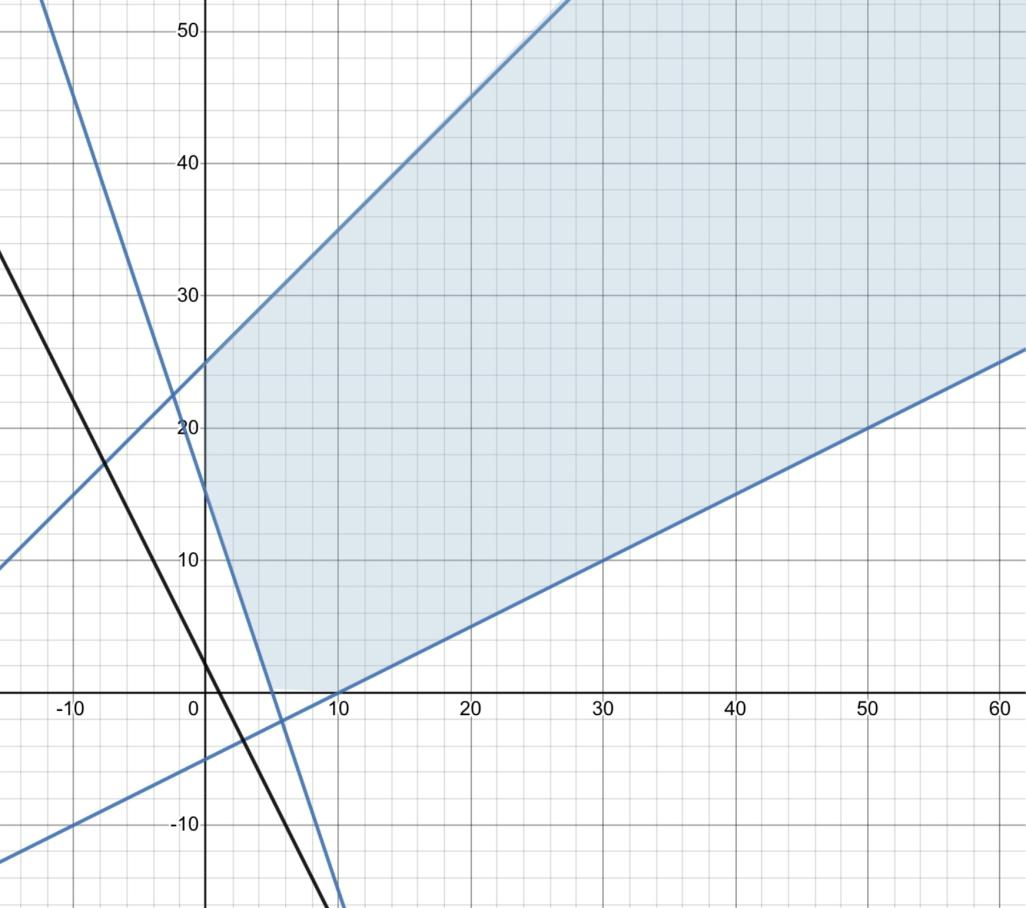
\includegraphics[width=5cm,right]{images/IMG_unbeschrankte_Losung.jpeg}
\\\\
Nichtnegativitätsbedingung:
\begin{math}1 <= 0, x_2 <= 0 \end{math}\\
\begin{table}[h]
\begin{tabular}{|l|l|l|l|l|l|l|}
\hline
\rowcolor[HTML]{C0C0C0} 
Zeile                     & $x_1$                         & $x_2$                          & $s_1$                        & $s_2$                        & $s_3$                        & RS \\ \hline
\cellcolor[HTML]{C0C0C0}1 & \cellcolor[HTML]{96FFFB}6  & \cellcolor[HTML]{FFFFFF}-12 & \cellcolor[HTML]{FFFFFF}1 & \cellcolor[HTML]{FFFFFF}0 & \cellcolor[HTML]{FFFFFF}0 & 60 \\ \hline
\cellcolor[HTML]{C0C0C0}2 & \cellcolor[HTML]{FFFFFF}-2 & \cellcolor[HTML]{FFFFFF}2   & \cellcolor[HTML]{FFFFFF}0 & \cellcolor[HTML]{FFFFFF}1 & \cellcolor[HTML]{FFFFFF}0 & 50 \\ \hline
\cellcolor[HTML]{C0C0C0}3 & \cellcolor[HTML]{FFFFFF}-3 & \cellcolor[HTML]{FFFFFF}1   & \cellcolor[HTML]{FFFFFF}0 & \cellcolor[HTML]{FFFFFF}0 & \cellcolor[HTML]{FFFFFF}1 & 15 \\ \hline
\cellcolor[HTML]{C0C0C0}Z & -10                        & -5                          & 0                         & 0                         & 0                         & 0  \\ \hline
\end{tabular}
\end{table}
\\
\begin{table}[!ht]
\begin{tabular}{|l|l|l|l|l|l|l|l|}
\hline
\rowcolor[HTML]{C0C0C0} 
Zeile                     & $x_1$                        & $x_2$                                  & $s_1$                          & $s_2$                        & $s_3$                        & RS  & Rechnung                \\ \hline
\cellcolor[HTML]{C0C0C0}1 & \cellcolor[HTML]{FFFFFF}1 & \cellcolor[HTML]{FFFFFF}\textbf{-2} & \cellcolor[HTML]{FFFFFF}1/6 & \cellcolor[HTML]{FFFFFF}0 & \cellcolor[HTML]{FFFFFF}0 & 10  & (wurde durch 6 geteilt) \\ \hline
\cellcolor[HTML]{C0C0C0}2 & \cellcolor[HTML]{FFFFFF}0 & \cellcolor[HTML]{FFFFFF}\textbf{-2} & \cellcolor[HTML]{FFFFFF}1/3 & \cellcolor[HTML]{FFFFFF}1 & \cellcolor[HTML]{FFFFFF}0 & 70  & +2*(Zeile 1)            \\ \hline
\cellcolor[HTML]{C0C0C0}3 & \cellcolor[HTML]{FFFFFF}0 & \cellcolor[HTML]{FFFFFF}\textbf{-5} & \cellcolor[HTML]{FFFFFF}1/2 & \cellcolor[HTML]{FFFFFF}0 & \cellcolor[HTML]{FFFFFF}1 & 45  & +3*(Zeile 1)            \\ \hline
\cellcolor[HTML]{C0C0C0}Z & 0                         & \textbf{-25}                        & 5/3                         & 0                         & 0                         & 100 & +10*(Zeile 1)           \\ \hline
\end{tabular}
\end{table}
\\
In diesem Beispiel kann der erste Iterationsschritt noch normal ausgeführt werden. Bei dem zweiten Iterationsschritt stößt man jedoch auf ausschließlich negative Werte in der Pivotspalte - somit kann keine optimale Lösung ermittelt werden.
\\
\textbf{Mehrere optimale Lösungen (unendlich viele Lösungen):}\\
In diesem Fall kann es mehrere optimale Lösungen des Optimierungsproblems geben. Dies wird im Optimaltableau erkennbar, wenn mindestens ein Wert in der Zeile der Zielfunktion einer Nichtbasisvariablen den Wert Null hat. Nimmt man diese mit in die Basis auf, ergibt sich eine weitere optimale Lösung.
\\
\textbf{Beispiel:}\\
Zielfunktion: max \begin{math}Z = 3*x_1+3*x_2\end{math}\\
Nebenbedingungen:\\
\begin{math}
3*x_1+3*x_2 <= 60\\
-1*x_1+1*x_2 <= 15\\
1*x_1 <= 15\\
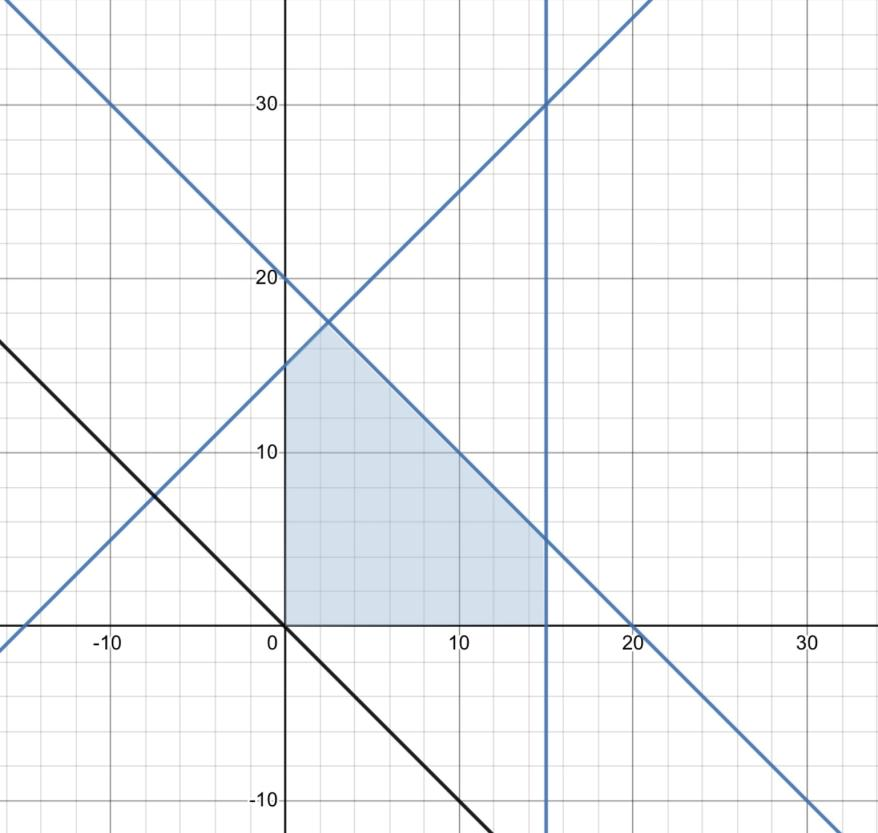
\includegraphics[width = 5cm, right]{images/IMG_unendlich_viele_Losungen.jpeg}
\end{math}\\
Nichtnegativitätsbedingung:\\
\begin{math}
x_1 >= 0, x_2 >= 0
\end{math}
\\
\begin{table}[!ht]
\begin{tabular}{|l|l|l|l|l|l|l|}
\hline
\rowcolor[HTML]{C0C0C0} 
Zeile                     & $x_1$                         & $x_2$                        & $s_1$                        & $s_2$                        & $s_3$                        & RS \\ \hline
\cellcolor[HTML]{C0C0C0}1 & \cellcolor[HTML]{FFFFFF}3  & \cellcolor[HTML]{FFFFFF}3 & \cellcolor[HTML]{FFFFFF}1 & \cellcolor[HTML]{FFFFFF}0 & \cellcolor[HTML]{FFFFFF}0 & 60 \\ \hline
\cellcolor[HTML]{C0C0C0}2 & \cellcolor[HTML]{FFFFFF}-1 & \cellcolor[HTML]{FFFFFF}1 & \cellcolor[HTML]{FFFFFF}0 & \cellcolor[HTML]{FFFFFF}1 & \cellcolor[HTML]{FFFFFF}0 & 15 \\ \hline
\cellcolor[HTML]{C0C0C0}3 & \cellcolor[HTML]{DAE8FC}1  & \cellcolor[HTML]{FFFFFF}0 & \cellcolor[HTML]{FFFFFF}0 & \cellcolor[HTML]{FFFFFF}0 & \cellcolor[HTML]{FFFFFF}1 & 15 \\ \hline
\cellcolor[HTML]{C0C0C0}Z & -3                         & -3                        & 0                         & 0                         & 0                         & 0  \\ \hline
\end{tabular}
\end{table}
\\
\begin{table}[!ht]
\begin{tabular}{|l|l|l|l|l|l|l|l|}
\hline
\rowcolor[HTML]{C0C0C0} 
Zeile                     & $x_1$                        & $x_2$                        & $s_1$                        & $s_2$                        & $s_3$                         & RS & Rechnung     \\ \hline
\cellcolor[HTML]{C0C0C0}1 & \cellcolor[HTML]{FFFFFF}0 & \cellcolor[HTML]{CBCEFB}3 & \cellcolor[HTML]{FFFFFF}1 & \cellcolor[HTML]{FFFFFF}0 & \cellcolor[HTML]{FFFFFF}-3 & 15 & -3*(Zeile 3) \\ \hline
\cellcolor[HTML]{C0C0C0}2 & \cellcolor[HTML]{FFFFFF}0 & \cellcolor[HTML]{FFFFFF}1 & \cellcolor[HTML]{FFFFFF}0 & \cellcolor[HTML]{FFFFFF}1 & \cellcolor[HTML]{FFFFFF}1  & 30 & +(Zeile 3)   \\ \hline
\cellcolor[HTML]{C0C0C0}3 & \cellcolor[HTML]{FFFFFF}1 & \cellcolor[HTML]{FFFFFF}0 & \cellcolor[HTML]{FFFFFF}0 & \cellcolor[HTML]{FFFFFF}0 & \cellcolor[HTML]{FFFFFF}1  & 15 &              \\ \hline
\cellcolor[HTML]{C0C0C0}Z & 0                         & -3                        & 0                         & 0                         & 3                          & 45 & +3*(Zeile 3) \\ \hline
\end{tabular}
\end{table}
\\
\begin{table}[!ht]
\begin{tabular}{|l|l|l|l|l|l|l|l|}
\hline
\rowcolor[HTML]{C0C0C0} 
Zeile                     & $x_1$ & $x_2$ & $s_1$   & $s_2$ & $s_3$ & RS & Rechnung                \\ \hline
\rowcolor[HTML]{FFFFFF} 
\cellcolor[HTML]{C0C0C0}1 & 0  & 1  & 1/3  & 0  & -1 & 5  & (wurde durch 3 geteilt) \\ \hline
\rowcolor[HTML]{FFFFFF} 
\cellcolor[HTML]{C0C0C0}2 & 0  & 0  & -1/3 & 1  & 2  & 25 & -(Zeile 1)              \\ \hline
\rowcolor[HTML]{FFFFFF} 
\cellcolor[HTML]{C0C0C0}3 & 1  & 0  & 0    & 0  & 1  & 15 &                         \\ \hline
\rowcolor[HTML]{FFFFFF} 
\cellcolor[HTML]{C0C0C0}Z & 0  & 0  & 1    & 0  & 0  & 60 & +3*(Zeile 1)            \\ \hline
\end{tabular}
\end{table}
\\
Würde man diesen Fall graphisch betrachten, wäre erkennbar, dass die Zielfunktion parallel zu einer Restriktion verläuft. Hier gibt es zwei Punkte, die gleichermaßen optimal sind. Alle Werte, welche zwischen diesen beiden Punkten liegen, sind dann ebenso optimal.\\
\textbf{Keine zulässige Lösung: }\\
Es gibt keine zulässige Lösung, wenn der zulässige Bereich leer ist. Zu diesem Fall kommt es, wenn sich zwei oder mehr Nebenbedingungen widersprechen.\\
Beispiel:\\
Zielfunktion: \begin{math}max Z = 6*x_1+4*x_2\end{math}\\
Nebenbedingungen:\\
\begin{math}
1/3*x_1+1/2*x_2 <= 20\\
2*x_1+1*x_2 <= 80\\
1*x_1+2*x_2 >= 90\\
\end{math}
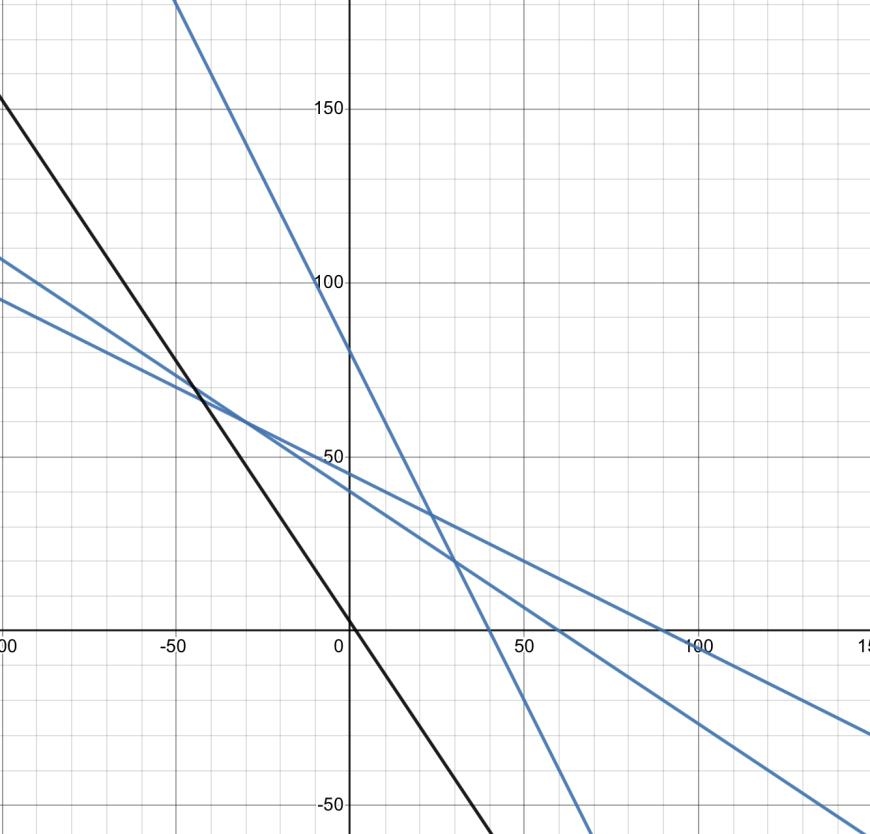
\includegraphics[width = 5cm, right]{images/IMG_keine_Losung.jpeg}
Nichtnegativitätsbedingung:\\
\begin{math}
x_1 >= 0, x_2>= 0\\
\end{math}
Aufgrund der Größer-Gleich-Bedingung muss im Tableau eine künstliche Variable s’3 angelegt werden. Diese muss in den folgenden Iterationen herausgerechnet werden.\\
\begin{table}[!ht]
\begin{tabular}{|l|l|l|l|l|l|l|l|}
\hline
\rowcolor[HTML]{C0C0C0} 
Zeile                      & $x_1$                          & $x_2$                          & $s_1$                        & $s_2$                        & $s_3$                        & s`3 & RS  \\ \hline
\cellcolor[HTML]{C0C0C0}1  & \cellcolor[HTML]{FFFFFF}1/3 & \cellcolor[HTML]{CBCEFB}1/2 & \cellcolor[HTML]{FFFFFF}1 & \cellcolor[HTML]{FFFFFF}0 & \cellcolor[HTML]{FFFFFF}0 & 0   & 20  \\ \hline
\cellcolor[HTML]{C0C0C0}2  & \cellcolor[HTML]{FFFFFF}2   & \cellcolor[HTML]{FFFFFF}1   & \cellcolor[HTML]{FFFFFF}0 & \cellcolor[HTML]{FFFFFF}1 & \cellcolor[HTML]{FFFFFF}0 & 0   & 80  \\ \hline
\cellcolor[HTML]{C0C0C0}3  & \cellcolor[HTML]{FFFFFF}1   & \cellcolor[HTML]{FFFFFF}2   & \cellcolor[HTML]{FFFFFF}0 & \cellcolor[HTML]{FFFFFF}0 & \cellcolor[HTML]{FFFFFF}1 & -1  & 90  \\ \hline
\cellcolor[HTML]{C0C0C0}Z  & \cellcolor[HTML]{FFFFFF}-6  & \cellcolor[HTML]{FFFFFF}-4  & \cellcolor[HTML]{FFFFFF}0 & \cellcolor[HTML]{FFFFFF}0 & \cellcolor[HTML]{FFFFFF}0 & 0   & 0   \\ \hline
\cellcolor[HTML]{C0C0C0}Z2 & -1                          & -2                          & 0                         & 0                         & 0                         & 1   & -90 \\ \hline
\end{tabular}
\end{table}
\\
\begin{table}[!ht]
\begin{tabular}{|l|l|l|l|l|l|l|l|l|}
\hline
\rowcolor[HTML]{C0C0C0} 
Zeile                      & $x_1$                            & $x_2$                        & $s_1$                           & $s_2$                        & $s_3$                        & s`3 & RS  & Rechnung                  \\ \hline
\cellcolor[HTML]{C0C0C0}1  & \cellcolor[HTML]{FFFFFF}2/3   & \cellcolor[HTML]{FFFFFF}1 & \cellcolor[HTML]{FFFFFF}1/2  & \cellcolor[HTML]{FFFFFF}0 & \cellcolor[HTML]{FFFFFF}0 & 0   & 40  & (wurde durch 1/2 geteilt) \\ \hline
\cellcolor[HTML]{C0C0C0}2  & \cellcolor[HTML]{FFFFFF}4/3   & \cellcolor[HTML]{FFFFFF}0 & \cellcolor[HTML]{FFFFFF}-1/2 & \cellcolor[HTML]{FFFFFF}1 & \cellcolor[HTML]{FFFFFF}0 & 0   & 40  & -(Zeile 1)                \\ \hline
\cellcolor[HTML]{C0C0C0}3  & \cellcolor[HTML]{FFFFFF}-1/3  & \cellcolor[HTML]{FFFFFF}0 & \cellcolor[HTML]{FFFFFF}-1   & \cellcolor[HTML]{FFFFFF}0 & \cellcolor[HTML]{FFFFFF}1 & -1  & 10  & -2*(Zeile 1)              \\ \hline
\cellcolor[HTML]{C0C0C0}Z  & \cellcolor[HTML]{FFFFFF}-10/3 & \cellcolor[HTML]{FFFFFF}0 & \cellcolor[HTML]{FFFFFF}2    & \cellcolor[HTML]{FFFFFF}0 & \cellcolor[HTML]{FFFFFF}0 & 0   & 160 & +4*(Zeile 1)              \\ \hline
\cellcolor[HTML]{C0C0C0}Z2 & 1/3                           & 0                         & 1                            & 0                         & 0                         & 1   & -10 & +2*(Zeile 1)              \\ \hline
\end{tabular}
\end{table}
\\
Die künstliche Variable lässt sich nicht herausrechnen, da in der Z2 Zeile keine negativen Werte mehr vorhanden sind. Die Zeile Z2 und die Zeile 3 schließen sich gegenseitig aus, wodurch kein Bereich gefunden werden kann, in dem ein valides Optimum existiert. Es gibt für dieses Optimierungsproblem also keine zulässige Lösung.\\
\textbf{Degenerierte Lösung: }\\
In diesem Fall existieren mehrere optimale Lösungen, da eine oder mehrere Basisvariablen bereits von Beginn an Null sind. Dadurch kommt es zu keiner Veränderung der rechten Seite des Tableaus, wenn ein Iterationsschritt ausgeführt wird.\\
\textbf{Beispiel: }\\
Zielfunktion: max Z = 2*$x_1$+2*$x_2$\\
\\
Nebenbedingungen:\\
\begin{math}
2*x_1 <= 60\\
4*x_1-4*x_2 <= 0\\
\end{math}
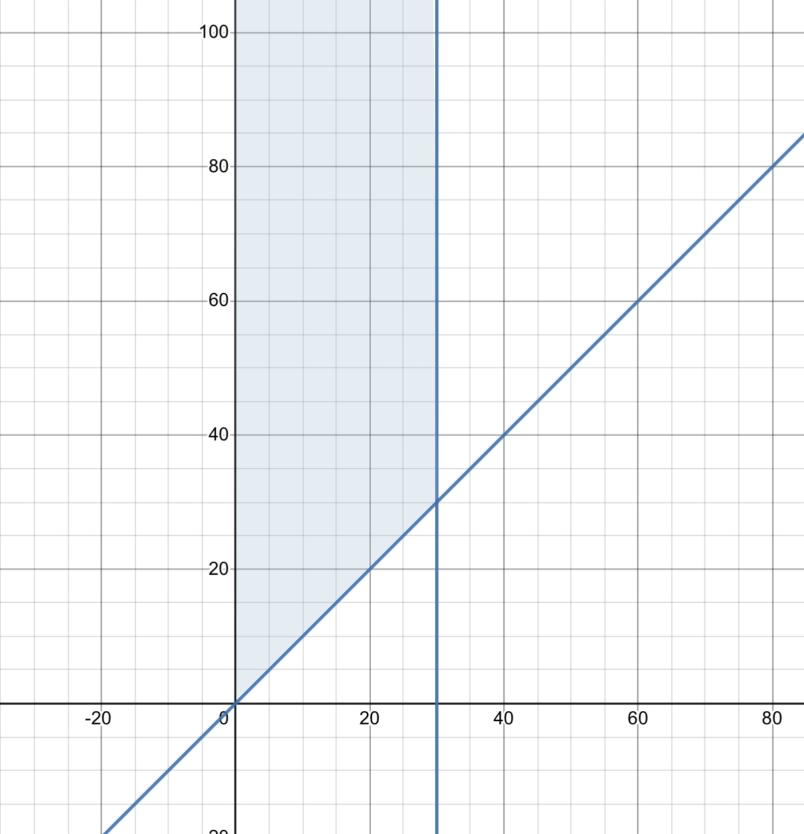
\includegraphics[width=5cm,right]{images/IMG_degenerierte_Losung.jpeg}
Nichtnegativitätsbedingung:\\
\begin{math}
x_1 >= 0, x_2 >= 0
\end{math}
\\
\begin{table}[!ht]
\begin{tabular}{|l|l|l|l|l|l|}
\hline
\rowcolor[HTML]{C0C0C0} 
Zeile                     & $x_1$                       & $x_2$ & $s_1$ & $s_2$ & RS \\ \hline
\rowcolor[HTML]{FFFFFF} 
\cellcolor[HTML]{C0C0C0}1 & 2                         & 0  & 1  & 0  & 60 \\ \hline
\rowcolor[HTML]{FFFFFF} 
\cellcolor[HTML]{C0C0C0}2 & \cellcolor[HTML]{CBCEFB}4 & -4 & 0  & 1  & 0  \\ \hline
\rowcolor[HTML]{FFFFFF} 
\cellcolor[HTML]{C0C0C0}Z & -2                        & -2 & 0  & 0  & 0  \\ \hline
\end{tabular}
\end{table}
\\
\begin{table}[!ht]
\begin{tabular}{|
>{\columncolor[HTML]{C0C0C0}}l |
>{\columncolor[HTML]{FFFFFF}}l |
>{\columncolor[HTML]{FFFFFF}}l |
>{\columncolor[HTML]{FFFFFF}}l |
>{\columncolor[HTML]{FFFFFF}}l |
>{\columncolor[HTML]{FFFFFF}}l |l|}
\hline
Zeile & \cellcolor[HTML]{C0C0C0}$x_1$ & \cellcolor[HTML]{C0C0C0}$x_2$ & \cellcolor[HTML]{C0C0C0}$s_1$ & \cellcolor[HTML]{C0C0C0}$s_2$ & \cellcolor[HTML]{C0C0C0}RS & \cellcolor[HTML]{C0C0C0}Rechnung \\ \hline
1     & 0                          & 2                          & 1                          & -1/2                       & 60                         & -2*(Zeile 2)                     \\ \hline
2     & 1                          & -1                         & 0                          & 1/4                        & 0                          & (wurde durch 4 geteilt)          \\ \hline
Z     & 0                          & -4                         & 0                          & 1/2                        & 0                          & +2*(Zeile 2)                     \\ \hline
\end{tabular}
\end{table}\\
Wie in diesem Beispiel deutlich wird, verändert sich die rechte Seite nicht. Somit gibt es für dieses Problem mehrere optimale Lösungen.









\section{Aufgabenstellung}
Nachdem wir an einem einfachen Beispiel den Simplex-Algorithmus und seine Sonderfälle dargestellt haben, wenden wir uns der Aufgabenstellung zu.
Hierbei geht es um ein Minimierungsproblem mit mehreren Nebenbedingungen. 
\subsection{Ziele des Projekts}
Die Aufgabe ist das Optimieren einer Personaleinsatzplanung.\\
Ein metallverarbeitendes Unternehmen in Oberberg benötigt für die Produktion -rund um die Uhr- Arbeiter.\\
Jeder Arbeiter arbeitet 4 Stunden, macht eine gewerkschaftliche Stunde Pause und arbeitet danach weitere 4 Stunden.\\
Die Arbeitszeit kann zu jeder beliebigen Stunde beginnen und wird mit 10€/Stunde bezahlt, es gibt einen Zuschlag von 2,50€/Stunde für Schichten in der Nacht von 10 Uhr abends bis 6 Uhr morgens.\\
\\
Die hier gegebenen Nebenbedingungen sind der Bedarf an Arbeitern zu bestimmten Uhrzeiten.\\
\\\\
12 Uhr nachts bis 6 Uhr morgens mindestens 2\\
6 Uhr morgens bis 10 Uhr morgens mindestens 8\\
10 Uhr morgens bis 12 Uhr mittags mindestens 4\\
12 Uhr nachmittags bis 4 Uhr nachmittags mindestens 3\\
4 Uhr nachmittags bis 6 Uhr nachmittags mindestens 6\\
6 Uhr nachmittags bis 10 Uhr abends mindestens 5\\
10 Uhr abends bis 12 Uhr nachts mindestens 3\\
\\\\
Die Zielfunktion ergibt sich aus dem Lohn, der für die jeweilige Schicht gezahlt werden muss (Koeffizient) und der Anzahl der Arbeiter, die für diese Schicht eingestellt werden müssen $(x_1-x{24})$.\\
Daraus resultiert folgende Zielfunktion: $z = 90*x_1 + 90*x_2 + 87.5*x_3 + 85*x_4 + 82.5*x_5 + 80*x_6 + 80*x_7 + 80*x_8 + 80*x_9 + 80*x_{10} + 80*x_{11} + 80*x_{12} + 80*x_{13} + 82.5*x_{14} + 85*x_{15} + 87.5*x_{16} + 90*x_{17} + 90*x_{18} + 92.5*x_{19} + 95*x_{20} + 97.5*x_{21} + 97.5*x_{22} + 95*x_{23} + 92.5*x_{24}$


\section{Zusammenfassung }

Zusammengefasst kann man sagen, dass man einige Probleme mit dem Simplex-verfahren lösen kann, sich jedoch nicht auf dieses verlassen sollte, da die Nebenbedingungen nicht immer Ideal und statisch sind und man hier auch nur Idealfälle ausrechnet. Das Problem hierbei ist, dass, je dynamischer die Nebenbedingungen werden, desto höher wird die benötigte Rechenleistung, sodass in großen Firmen oder bei anderen Problemen sich das ausrechnen eines theoretischen Idealfalls nicht mehr lohnt, da von vornherein klar ist, dass dieser höchstwahrscheinlich nicht eingehalten werden kann. \\
Bei einer kleineren menge an Nebenbedingungen wie in diesem Problem, bei welchem davon ausgegangen wird, dass niemand Krank wird, an bestimmten Tagen Termine hat und immer die gleiche Zeit auf der Arbeit verbringt, kann man das Ergebnis als grobe Richtlinie verwenden, jedoch wird dieses Ergebnis immer unrealistischer, je realistischer die Bedingungen werden.

\subsection{Kurs Reflexion}

Der Gruppe hat das Rechnen mit dem Simplex-verfahren spaß gemacht und es war äußerst interessant ${\displaystyle \mathrm {L\!\!^{{}_{A}}\!\!\!\!\!\;\;T\!_{\displaystyle E}\!X} }$, die Simplex-Funktionen von Excel kennen zu lernen sowie die Idealfälle graphisch darzustellen.

{\bf Note:} Für spätere Notizen



\end{document}
